\documentclass[sigconf]{acmart}
\usepackage{algorithm}
\usepackage{algpseudocode}
\usepackage{comment}


% \setcopyright{acmlicensed}
% \copyrightyear{2024}
% \acmYear{2024}
% \acmDOI{XXXXXXX.XXXXXXX}

\acmConference{Geometry Data Analysis}{December 2024}{Paris, France}

\acmISBN{978-1-4503-XXXX-X/18/06}
\begin{document}
%%
%% The "title" command has an optional parameter,
%% allowing the author to define a "short title" to be used in page headers.
\title{Analysis over the Vector Heat Method}

%%
%% The "author" command and its associated commands are used to define
%% the authors and their affiliations.
%% Of note is the shared affiliation of the first two authors, and the
%% "authornote" and "authornotemark" commands
%% used to denote shared contribution to the research.
\author{Ícel Viñals Pierigé}
\affiliation{%
  \institution{\'Ecole nationale des Ponts et Chaussées}
  \city{Champs-sur-Marne}
  \country{France}}
\email{icel.vinals-pierige@enpc.fr}

\author{Cécile Liu}
\affiliation{%
  \institution{\'Ecole nationale des Ponts et Chaussées}
  \city{Champs-sur-Marne}
  \country{France}}
\email{cecile.liu@enpc.fr}

\author{Nicolas Sereyjol-Garros}
\affiliation{%
  \institution{\'Ecole nationale des Ponts et Chaussées}
  \city{Champs-sur-Marne}
  \country{France}}
\email{nicolas.sereyjol-garros@enpc.fr}


\begin{abstract}
  A clear and well-documented \LaTeX\ document is presented as an
  article formatted for publication by ACM in a conference proceedings
  or journal publication. Based on the ``acmart'' document class, this
  article presents and explains many of the common variations, as well
  as many of the formatting elements an author may use in the
  preparation of the documentation of their work.
\end{abstract}

%%
%% The code below is generated by the tool at http://dl.acm.org/ccs.cfm.
%% Please copy and paste the code instead of the example below.
%%
\begin{CCSXML}
<ccs2012>
   <concept>
       <concept_id>10010147.10010371.10010396.10010402</concept_id>
       <concept_desc>Computing methodologies~Shape analysis</concept_desc>
       <concept_significance>500</concept_significance>
       </concept>
   <concept>
       <concept_id>10002950.10003714.10003715.10003750</concept_id>
       <concept_desc>Mathematics of computing~Discretization</concept_desc>
       <concept_significance>500</concept_significance>
       </concept>
   <concept>
       <concept_id>10002950.10003714.10003727.10003729</concept_id>
       <concept_desc>Mathematics of computing~Partial differential equations</concept_desc>
       <concept_significance>500</concept_significance>
       </concept>
 </ccs2012>
\end{CCSXML}

\ccsdesc[500]{Computing methodologies~Shape analysis}
\ccsdesc[500]{Mathematics of computing~Discretization}
\ccsdesc[500]{Mathematics of computing~Partial differential equations}

%%
%% Keywords. The author(s) should pick words that accurately describe
%% the work being presented. Separate the keywords with commas.
\keywords{discrete differential geometry, parallel
transport, velocity extrapolation, logarithmic map, exponential map, Karcher
mean, geometric median}

\received{20 February 2007}
\received[revised]{12 March 2009}
\received[accepted]{5 June 2009}

%%
%% This command processes the author and affiliation and title
%% information and builds the first part of the formatted document.
\maketitle

\section{Introduction}

\section{Parallel Transport}

\subsection{Preliminaries: Covariant Derivative}
Transporting a vector in an euclidean space into a constant vector field is trivial. However, this operation done on a curved manifold, like for example a a curved surface in a 3D space, requires to carefully change the orientation of the vector to keep the vectors as "parallel" as possible. Indeed, the vectors must reamains in the tangent spaces of the surface while the normals of the tangent spaces change. When parallel transporting a vector along the shortest geodesic path, the vector rate of change should be only normal to the surface. 

More formally, to keep the vector as parallel as possible, the covariant derivative should be equal to 0 \cite{youtube_video}. The covariant derivative along a direction $\vec{w} $ is the rate of change of the vector in the direction $\vec{w}$ with the normal component substracted (Eq. \ref{eq:covariant derivative}) i.e. the orthogonal projection of the usual derivative onto the tangent space.

\begin{equation}
  \nabla_{\vec{W}}\vec{v}:=\frac{d\vec{v}}{d\vec{w}}-\vec{n}=0
  \label{eq:covariant derivative}
\end{equation}

\subsection{Parallel Transport of a vector}

transport vector along shortest path/geodesic

\subsection{Applications}
Parallel transporting a vector can be very useful in a wide range of applications where algorithm can build on it. It includes for example extrapolating velocities, mapping texture on a curved surface by defining a map relative to aspecified point, finding the center of a set of points on a curved surface, or even partition a shape whith a Voronoi diagram. Those methods would greatly benefit from a fast and accurate parallel transport method.

\subsubsection{Extrapolating velocities}
Parallel transport can be used to extrapolate velocities on a curved surface. To advect quantities like color or temperature, a global and well behaved velocity field on the surface is needed. The parallel transport can be used to extrapolate the velocity field from a set of points on the surface on the whole surface.

\subsubsection{logarithmic map}
Defining a map on a curved surface can be crucial for several tasks in geometry processing, like interactive shape editing or texture decaling. A map, called logarithmic map, can be easily commputed thanks to parallel transport. The logarithmic map is simply a map relative to a specified point on the surface with polar coordinates. 

It can be defined as the inverse operation of the exponential map. Let the point $x$ be on a closed surface $M$, the exponential map $\exp_x (rv)$ outputs the point $y\in M$ by starting from $x$ and walking in the tangent direction $v$ along a geodesic for a distance $r$. The logarithmic map $\log_x(y)$ is the inverse operation, it outputs the tangent vector $v$ and the smallest distance $r$ so that $\exp_x (rv)=y$. The vector $v$ can be associated with an angle $\varphi$ to define a polar coordinate system.

While $r$ is easily defined as the geodesic distance between $y$ and $x$, $\varphi$ is defined as the angle between an "horizontal" vector field and the radial vector field emenating from the origin $x$. The radial vector field is the gradient of the geodesic distance from $x$. The horizontal vector field is the parallel transport on the all shape of any vector at x. This explain why parallel transport is needed to define the logarithmic map. 

\begin{figure}[h]
  \centering
  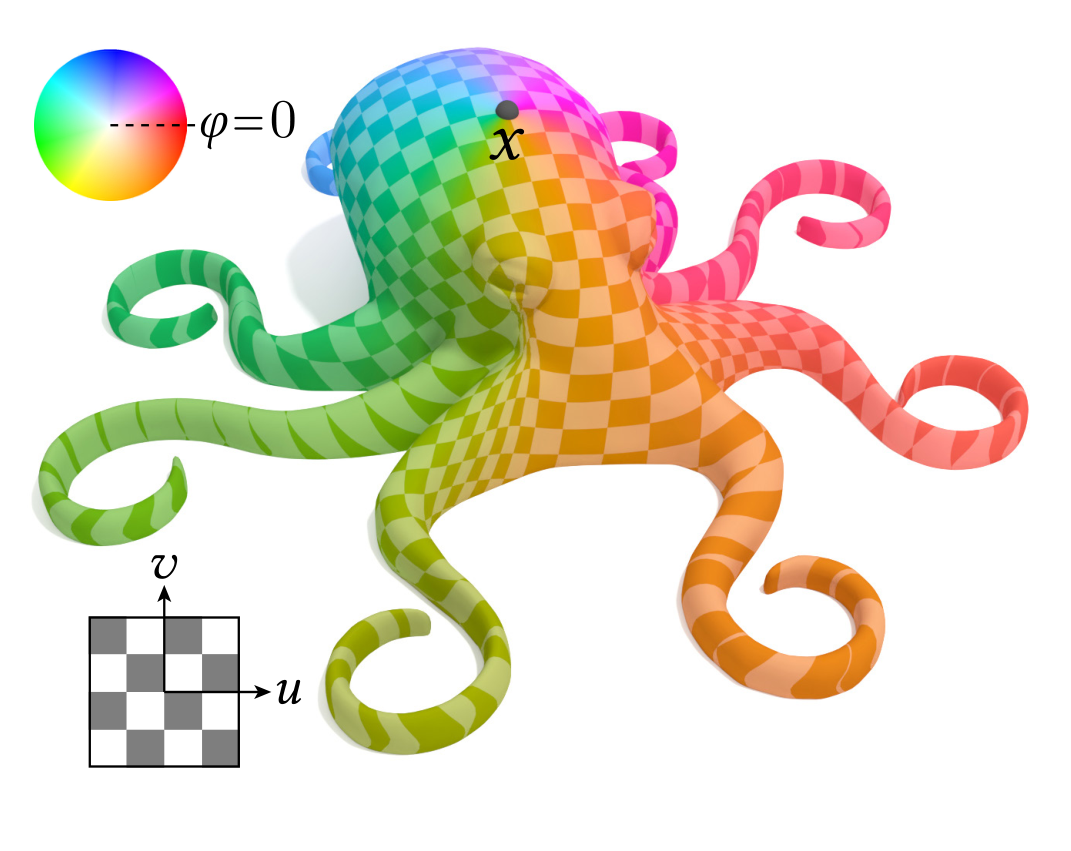
\includegraphics[width=0.5\textwidth]{img/logmap_paper.png}
  \caption{\textbf{Logarithmic map on a curved surface}. \textmd{The logarithmic map provides a coordinate system on the surface with respect to an origin and a choice of an initial unit vector to define $\varphi$.}}
  \label{fig:logarithmic_map}
\end{figure}


\subsubsection{Karcher/Fréchet means and geometric medians on general surfaces }
Notion of center by minimizing a distance to all points of the set. The Karcher mean is the point that minimizes the sum of the squared geodesic distances to all points of the set. The gradient at a point $x$ of the energy to minimize is just the sum of the logarithms $\log_x y_i$ of the points of the set. Iteratively update and rceompute logmap. 

\subsubsection{Voronoi diagram on surfaces}
Derived from the karcher mean, the Voronoi diagram on surfaces is a partition of the surface into regions that are closer to a given set of points than to any other point on the surface. 


\section{Methodologies}
Let $M$ be a Riemannian manifold with metric $g$. We denote by $d(x,y)$ the corresponding geodesic distance. 
The cut locus of a point $p$ on $M$ is the closure of the set of all other points on $M$ that are connected to $p$
by two or more distinct shortest geodesics. More generally, the cut locus of a closed set $X$ on $M$ is the closure of the set of 
all other points on the manifold connected to $X$ by two or more distinct shortest geodesics.
\subsection{Vector heat method}
The vector heat method \cite{sharp_vector_2019} is presented in algorithm \ref{algo1}: the vector heat equation is used to diffuse the input vector field and then the scalar heat vector is used to adjust the magnitude of the resulting vectors. Indeed, the vector heat equation gives vectors pointing to the right directions for small values of time $t$ but the magnitudes are wrong. 

\begin{algorithm}
\caption{Vector Heat Method} \label{algo1}
\begin{algorithmic}
\Require A vector field $X$ supported on a subset $\Omega \subset M$ of the domain $M$.
\Ensure A vector field $\overline{X}$ on all of $M$.
%\Input{A vector field $X$ supported on a subset $\Omega \subset M$ of the domain $M$.}
%\Output{A vector field $\overline{X}$ on all of $M$.}

\noindent \textbf{I.} Integrate the vector heat flow $\frac{d}{dt} Y_t = \Delta Y_t$ for time $t$, with $Y_0 = X$. \\

\textbf{II.} Integrate the scalar heat flow $\frac{d}{dt} u_t = \Delta u_t$ for time $t$, with $u_0 = |X|$. \\

\textbf{III.} Integrate the scalar heat flow $\frac{d}{dt} \phi_t = \Delta \phi_t$ for time $t$, with $\phi_0 = \mathbf{1}_{\Omega}$. \\

\textbf{IV.} Evaluate the vector field $\overline{X}_t = \frac{u_t Y_t}{\phi_t |Y_t|}$.
\end{algorithmic}
\end{algorithm}

\subsubsection{Step 1: get the right directions}
As mentioned earlier, the idea of the vector heat method is to use the vector heat equation 
\begin{equation} \label{eq:vector-heat}
  \frac{d}{dt} X_t = \Delta^\nabla X_t
  \end{equation}
to diffuse the initial vector field. The symbol $\Delta^\nabla$ denotes the connection Laplacian associated to the Levi-Civita connection $\nabla$. 
We now consider a fundamental solution to the heat equation: the \textbf{heat kernel} denoted by $k_t^\nabla$. $k_t^\nabla(x,y)$ describes how 
a vector at a single point $x$ will diffuse to all other points $y$ over time $t$. For $y$ not on the cut locus of $x$, the following asymptotic
expansion holds:
\begin{equation} \label{eq:asymptotic_expansion}
  k_t^\nabla(x, y) \sim \frac{e^{-\frac{d(x, y)^2}{4t}}}{(4 \pi t)^{n/2} j(x, y)^\frac{1}{2}} 
\left( \sum_{i=0}^{\infty} t^i \Psi_i(x, y) \right)
  \end{equation}
where the functions $\Psi_i$ are maps taking vector at $x$ to vectors at $y$. Most importantly, we have that the first function in this series 
is equal to:
$$\Psi_0(x,y) = P_{\gamma_{x\rightarrow y}}, $$ where $\gamma_{x \rightarrow y}$ is the shortest geodesic from $x$ to $y$ and $P_\gamma(X)$
denotes the parallel transport of X along $\gamma$. Thus, by taking $t\rightarrow 0$, the terms for which $i\neq 0$ vanish, so \textbf{the vector heat 
kernel is asymptotically equal up to a constant to the parallel transport along shortest paths.} This explains the step 1 of the algorithm, whose goal 
is to get the right directions of the parallel transport of the input vector field.
\subsubsection{Step 2: get the right magnitudes}
We use scalar interpolation to scale the vectors obtained in step 1 and get the right magnitudes. Assume we have a collection of sources
$p_1, \dots, p_n \in M$ and associated values $u_1, \dots, u_n \in \mathbb{R}$. We define the functions $u$ and $\Phi$ 
as the solutions of two independent heat equations with initial conditions:
\begin{align}
  u(t = 0, p) = \sum_{i = 1}^nu_i\delta_{p_i}(p) \label{eq:initial_condition_1}\\
  \Phi(t = 0, p) = \sum_{i=1}^n\delta_{p_i}(p) \label{eq:initial_condition_2}
\end{align}
We then take as interpolant of the right magnitudes 
\begin{equation}
  \overline{u}(t,p) = \frac{u(t,p)}{\Phi(t,p)}
\end{equation}
In the following, we generalize the source set to any subset $\Omega \subset M$
and so the initial conditions \ref{eq:initial_condition_1} and \ref{eq:initial_condition_2}
are slightly modified to 
\begin{align*}
  u(t=0, p) = | X(p) | \\
  \Phi(t=0, p) = \mathbf{1}_{\Omega}(p)
\end{align*}



\begin{comment}
\begin{algorithm}
\caption{An algorithm with caption}\label{alg:cap}
\begin{algorithmic}
\Require $n \geq 0$
\Ensure $y = x^n$
\State $y \gets 1$
\State $X \gets x$
\State $N \gets n$
\While{$N \neq 0$}
\If{$N$ is even}
    \State $X \gets X \times X$
    \State $N \gets \frac{N}{2}$  \Comment{This is a comment}
\ElsIf{$N$ is odd}
    \State $y \gets y \times X$
    \State $N \gets N - 1$
\EndIf
\EndWhile
\end{algorithmic}
\end{algorithm}
\end{comment}

\section{Experiences}

\subsection{Our set-up}
(icel)
\subsection{Scalar heat rebustess (different noise types)}
(icel)

\subsection{T's verifications with perfect results}
(nicolas)
https://hhoppe.com/geodesics.pdf

\subsection{Behavior at cut locus}
(cécile)
\subsection{Log-map recreation for postures}

\subsection{Preprocessing vs processing times}

\section{Limitations}
\section{Conclusion}




\section{BRAIN STORM:}
\begin{itemize}
  \item Test robustness with a custom mesh + noise (similar to what they did) and mesh+crossed triangles (shortcuts should break the results?)
  \item Test different step sizes (t's) verify that 1 seems to be the best
  \item Compare results numerically with 'perfect' algorithm from https://hhoppe.com/geodesics.pdf
  \item Find how to test with different data types (point clouds, triang meshes, poly meshes) and compare results (if possible in software without too much rewriting?)
  \item Try results on bad vs good triangulated meshes (to check if Delaunay works fine)
  \item Think about new possible applications? Videogames/3d animation?? 
  \item Check 2020 method to compute geodesics only by flipping triangles. One advantage seems to be that it works to find not only global shortest paths, but also local ones (if two points are next to each other, it can find the shortest path in the opposite direction by turning around)  https://dl.acm.org/doi/10.1145/3414685.3417839
  \item Test speed against fast marching method for scalar heat method
  \item Check behaviour at Cut locus and comment it
  \item Look for applications the Karcher mean
\end{itemize}
\bibliographystyle{ACM-Reference-Format}
\bibliography{ref}

\end{document}

\endinput
%%
%% End of file `sample-sigconf-authordraft.tex'.
